% Creación de una presentación en Beamer basada en tu trabajo de grado
\documentclass[aspectratio=169, xcolor={dvipsnames}, 10pt, spanish]{beamer}
\usepackage{multicol}
\usepackage[backend=bibtex,style=numeric]{biblatex}
\addbibresource{references.bib}

% Incluir las personalizaciones desde customizacoes.tex
% Pacotes
\usepackage{lipsum}
\usepackage{graphicx}
\usepackage{color}
\usepackage[table]{xcolor}
\usepackage{tikz}
\usepackage{tcolorbox}
\usepackage{amsmath}
\usepackage{amsfonts}
\usepackage{amssymb}
\usepackage{mathrsfs}
\usepackage{mathtools}
% \usepackage{enumitem} % Comentamos o eliminamos esta línea
\usepackage{float}
\usepackage[utf8]{inputenc}	
\usepackage[spanish]{babel}
\usepackage{caption}
\usepackage{hyperref}



% Theme choice:
\usetheme{CambridgeUS}

% Cores personalizadas
\definecolor{PROFMATgreen}{RGB}{0, 138, 163}
\definecolor{UFTgreen}{RGB}{0, 137, 124}
\definecolor{UFTblue}{RGB}{0, 84, 132}
\definecolor{UFTyellow}{RGB}{253, 185, 46}
\definecolor{UFTgray}{RGB}{132, 134, 136}

% Ativar numeração de tabelas
\setbeamertemplate{caption}[numbered]

% Ajustes de colores y estilos
\setbeamercolor*{structure}{bg=UFTgreen,fg=black}

\setbeamercolor*{palette primary}{fg=black,bg=PROFMATgreen}
\setbeamercolor*{palette secondary}{fg=white,bg=UFTblue}
\setbeamercolor*{palette tertiary}{fg=black,bg=UFTgreen}
\setbeamercolor*{palette quaternary}{fg=white,bg=black}

\setbeamercolor{section in toc}{fg=black,bg=white}
\setbeamercolor{alerted text}{fg=white}

\setbeamercolor*{item}{fg=PROFMATgreen}

\setbeamercolor{block title}{bg=UFTgreen,fg=white}
\setbeamercolor{block body}{bg=UFTgray!10,fg=black}

\setbeamercolor{titlelike}{fg=white, bg=UFTblue}
\setbeamercolor{frametitle}{bg=UFTgray!20,fg=UFTgreen}

% Personalizar la página de título
\setbeamertemplate{title page}{
    \vbox{}
\begin{minipage}{0.2\linewidth}
        \centering
        
\includegraphics[width=0.8\linewidth]{UD.png}
    \end{minipage}
    \hfill
    \begin{minipage}{0.2\linewidth}
        \centering
        
\includegraphics[width=0.8\linewidth]{BBVA.png}
    \end{minipage}
    
    %\vfill
    \vskip1em\par
    \begingroup
        \centering
        \begin{beamercolorbox}[sep=8pt,center,shadow=true,rounded=false]{title}
            \usebeamerfont{title}\inserttitle\par%
            \ifx\insertsubtitle\@empty%
            \else%
                \vskip0.25em%
                {\usebeamerfont{subtitle}\usebeamercolor[fg]{subtitle}\insertsubtitle\par}%
            \fi%
        \end{beamercolorbox}%
        \vskip1em\par
        \begin{beamercolorbox}[sep=6pt,center]{author}
            \usebeamerfont{author}\insertauthor
        \end{beamercolorbox}
        \vskip0.2em\par
        \begin{beamercolorbox}[sep=5pt,center]{advisor}
            \usebeamerfont{institute} \advisorname
        \end{beamercolorbox}
        \vskip0.2em\par
        \begin{beamercolorbox}[sep=5pt,center]{institute}
            \usebeamerfont{institute}\insertinstitute
        \end{beamercolorbox}
        \vskip0.2em\par
        \begin{beamercolorbox}[sep=5pt,center]{date}
            \usebeamerfont{institute}\insertdate
        \end{beamercolorbox}
        \vskip0.5em\par
    \endgroup
    \vfill
}

% Remover bordes redondeados de los bloques
\makeatletter
\setbeamertemplate{blocks}[default]
\makeatother


\setbeamercolor{bibliography entry author}{fg=black}
\setbeamertemplate{bibliography item}{\newblock}

\setbeamertemplate{frametitle continuation}{}

% Ajustes de separadores en figuras y tablas
\captionsetup[figure]{labelformat=simple, labelsep=endash, textformat=period, font=footnotesize}
\captionsetup[table]{labelformat=simple, labelsep=endash, textformat=period, font=footnotesize}

% Espaciado antes y después de las leyendas
\captionsetup[figure]{aboveskip=2pt, belowskip=0pt}
\captionsetup[table]{aboveskip=2pt, belowskip=0pt}

% Ajustes de guiones y tolerancia
\hyphenpenalty=10000
\tolerance=10000

% Personalización del estilo del índice
\setbeamertemplate{section in toc}[sections numbered]
\renewcommand{\thesection}{\textcolor{PROFMATgreen}{\arabic{section}}}
\renewcommand{\thesubsection}{\textcolor{PROFMATgreen}{\arabic{section}.\arabic{subsection}}}

\setbeamersize{text margin left=0.8cm, text margin right=0.8cm}


% Información del documento
\title[Extracción de Insights Clave para la Toma de Decisiones]{Extracción de Insights Clave para la Toma de Decisiones a partir de Comentarios Negativos de Detractores del Banco BBVA}
\subtitle{Trabajo de Grado Modalidad Pasantía}
\author[Wilson E. Jerez H.]{Wilson Eduardo Jerez Hernández}
\institute[Universidad Distrital]{Universidad Distrital Francisco José de Caldas}
\date{Diciembre 2024}

% Definir el nombre del director y codirector
\newcommand{\advisorname}{\textbf{Director:} Luis Alejandro Masmela Caita}
\newcommand{\codirectorname}{\textbf{Codirector:} John Pablo Calvo López}

% Personalización de bullets en listas
\setbeamertemplate{itemize item}{\color{UFTgreen}$\blacksquare$}
\setbeamertemplate{itemize subitem}{\color{UFTgreen}$\blacktriangleright$}
\setbeamertemplate{itemize subsubitem}{\color{UFTgreen}$\small\bullet$}

% Incluir los paquetes hyperref y url para manejar las URLs correctamente
\usepackage{hyperref}
\usepackage{url}

\begin{document}

% Slide de título
\begin{frame}
    \titlepage
\end{frame}

% Sumario
\begin{frame}[t]
    \frametitle{Contenido}
    \begin{multicols}{3}
    \tableofcontents
    \end{multicols}
\end{frame}

% Sección: Resumen
\section*{Resumen}
\begin{frame}{Resumen}
    Este trabajo presenta el desarrollo de un modelo de análisis de sentimientos basado en técnicas de \textbf{Machine Learning}, con el objetivo de clasificar y obtener \textit{insights} a partir de comentarios negativos emitidos por los detractores del Banco BBVA. El propósito principal es identificar áreas de mejora en los servicios del banco para aumentar la satisfacción del cliente y reducir el número de detractores. Para lograrlo, se emplea \textbf{procesamiento de lenguaje natural (NLP)} sobre datos textuales obtenidos de redes sociales y encuestas internas.
\end{frame}

% Sección: Palabras Clave
\begin{frame}{Palabras Clave}
    \begin{itemize}
        \item \textbf{Machine Learning}
        \item \textbf{Análisis de Sentimiento}
        \item \textbf{NLP}
        \item \textbf{BBVA}
        \item \textbf{Clientes Detractores}
    \end{itemize}
\end{frame}

% Sección: Agradecimientos
\section*{Agradecimientos}
\begin{frame}{Agradecimientos}
    Quiero agradecer profundamente a mi familia por su amor, paciencia y apoyo incondicional en cada paso de este camino.

    A mis docentes, especialmente a mi director Alejandro Masmela, por su orientación y confianza durante todo este proceso.

    Al semillero IPREA, gracias por darme la oportunidad de aprender y crecer en lo que más me apasiona.

    A mi Sangha, por ser siempre una fuente de tranquilidad, sabiduría y luz en mi vida.

    A John Calvo, gracias por tu guía, paciencia y enseñanzas. Tu apoyo fue clave para lograr el equilibrio entre mi crecimiento académico y personal.

    Este trabajo es fruto del esfuerzo de todos, y les estaré siempre agradecido.
\end{frame}

% Sección: Introducción
\section{Introducción}
\begin{frame}{Introducción}
    El sector bancario ha experimentado transformaciones profundas debido a la creciente digitalización, la evolución en las expectativas de los clientes y una competencia cada vez más feroz. En este entorno, la capacidad de captar y analizar la retroalimentación de los clientes se ha vuelto esencial para las entidades bancarias que desean adaptarse rápidamente a las demandas del mercado.

    \vfill
    Los comentarios negativos, en particular, representan una fuente valiosa de información, ya que pueden revelar problemas recurrentes o áreas de oportunidad que, si se abordan correctamente, podrían traducirse en una mayor satisfacción y fidelización de los clientes.
\end{frame}

\begin{frame}{Introducción (cont.)}
    En este contexto, \textbf{BBVA Colombia} ha tomado la iniciativa de implementar un modelo de análisis de sentimientos utilizando técnicas avanzadas de \textit{Machine Learning}. Este modelo se enfoca en la clasificación y análisis de los comentarios emitidos por los \textbf{detractores}, aquellos clientes que han expresado insatisfacción o frustración con los servicios ofrecidos.

    \vfill
    El objetivo principal de este enfoque es identificar de manera eficiente las áreas críticas de mejora, permitiendo a BBVA Colombia realizar ajustes estratégicos que mejoren la experiencia del cliente y reduzcan el índice de detractores.
\end{frame}

\begin{frame}{Introducción (cont.)}
    Para lograrlo, se emplea el \textbf{procesamiento de lenguaje natural (NLP)}, una rama de la inteligencia artificial que permite analizar y comprender grandes volúmenes de datos textuales de manera automatizada.

    \vfill
    Las fuentes de estos datos incluyen \textbf{redes sociales}, donde los clientes expresan sus opiniones de forma pública, y \textbf{encuestas internas} del banco, que proporcionan una visión más detallada y directa de las experiencias de los usuarios.

    \vfill
    A través de este análisis, BBVA Colombia busca convertir los comentarios negativos en oportunidades de mejora, fortaleciendo así su oferta de valor y consolidando su posición en un mercado altamente competitivo.
\end{frame}

% Sección: Objetivos
\section{Objetivos}
\subsection{Objetivo General}
\begin{frame}{Objetivo General}
    Desarrollar un modelo de análisis de sentimiento basado en técnicas de \textit{Machine Learning} que permita extraer \textbf{insights clave} a partir de los comentarios negativos emitidos por los detractores del Banco BBVA Colombia, con el fin de proporcionar información estratégica que facilite la toma de decisiones en la alta gerencia y contribuya a la mejora continua de los servicios ofrecidos.
\end{frame}

\subsection{Objetivos Específicos}
\begin{frame}{Objetivos Específicos}
    \begin{enumerate}
        \item \textbf{Transformación de comentarios en representaciones vectoriales}: Implementar el modelo \textbf{TfidfVectorizer} para convertir los comentarios negativos en representaciones vectoriales, identificando palabras y términos clave relacionados con áreas de insatisfacción.
        \item \textbf{Identificación de temas mediante Topic Modeling (LDA)}: Aplicar técnicas de \textbf{Latent Dirichlet Allocation (LDA)} para agrupar comentarios en tópicos relevantes.
    \end{enumerate}
\end{frame}

\begin{frame}{Objetivos Específicos (cont.)}
    \begin{enumerate}
        \setcounter{enumi}{2}
        \item \textbf{Evaluación de la coherencia del modelo}: Calcular valores de coherencia para distintos números de temas, garantizando que los temas extraídos sean consistentes.
        \item \textbf{Análisis de áreas críticas de insatisfacción}: Realizar un análisis profundo para determinar áreas con mayores niveles de insatisfacción y proporcionar recomendaciones claras.
    \end{enumerate}
\end{frame}

\begin{frame}{Objetivos Específicos (cont.)}
    \begin{enumerate}
        \setcounter{enumi}{4}
        \item \textbf{Visualización de resultados}: Generar visualizaciones que muestren la distribución de los temas, facilitando la comprensión y comunicación de los resultados.
        \item \textbf{Soporte para la toma de decisiones estratégicas}: Proporcionar información clave para orientar acciones correctivas y mejorar la experiencia del cliente.
    \end{enumerate}
\end{frame}

% Sección: Marco Teórico
\section{Marco Teórico}
\subsection{BBVA Colombia: Una Entidad Financiera Líder}
\begin{frame}{BBVA Colombia: Una Entidad Financiera Líder}
    BBVA Colombia es una destacada institución bancaria que forma parte del \textbf{Grupo BBVA}, uno de los conglomerados financieros más grandes del mundo. A lo largo de su historia, la entidad ha experimentado una notable evolución, marcada por adquisiciones estratégicas, innovaciones tecnológicas y un fuerte compromiso con el desarrollo sostenible \cite{2}.
\end{frame}

\subsubsection{Historia y Fundación}
\begin{frame}{Historia y Fundación}
    \begin{itemize}
        \item Fundada en 1956 como \textbf{Banco Ganadero}, enfocada en el desarrollo agropecuario en Colombia.
        \item En 1996, el \textbf{Banco Bilbao Vizcaya (BBV)} adquirió el 34,7\% de las acciones, iniciando su expansión en el país \cite{2}.
    \end{itemize}
\end{frame}

\subsubsection{Evolución y Fusión}
\begin{frame}{Evolución y Fusión}
    \begin{itemize}
        \item En 1998, BBV incrementó su participación adquiriendo un 15\% adicional de acciones.
        \item La entidad pasó a llamarse \textbf{BBV Banco Ganadero}.
        \item En 1999, la fusión entre BBV y Argentaria dio lugar a \textbf{BBVA}.
        \item En 2004, se renombró formalmente como \textbf{BBVA Colombia} \cite{2}.
    \end{itemize}
\end{frame}

\subsubsection{Adquisición de Granahorrar y Consolidación}
\begin{frame}{Adquisición de Granahorrar y Consolidación}
    \begin{itemize}
        \item En 2005, BBVA Colombia adquirió \textbf{Granahorrar}, entidad enfocada en el mercado hipotecario.
        \item En 2006, se fusionaron bajo la marca BBVA Colombia.
        \item Consolidó su liderazgo en el sector hipotecario y amplió su presencia en el país \cite{2}.
    \end{itemize}
\end{frame}

\subsubsection{Innovación y Transformación Digital}
\begin{frame}{Innovación y Transformación Digital}
    \begin{itemize}
        \item Pionera en la transformación digital del sector bancario en Colombia.
        \item Promueve el uso de canales digitales para mejorar la experiencia del cliente.
        \item Campaña \textbf{Uga Uga} para impulsar el cambio hacia la banca digital \cite{3}.
    \end{itemize}
\end{frame}

\subsubsection{Inversión en Tecnología y Desarrollo Sostenible}
\begin{frame}{Inversión en Tecnología y Desarrollo Sostenible}
    \begin{itemize}
        \item En 2023, inversión récord de más de \$235.000 millones en tecnología.
        \item Renovación de aplicaciones móviles y expansión de productos digitales.
        \item Crecimiento del 98\% en financiación sostenible, movilizando \$6,7 billones \cite{4}.
    \end{itemize}
\end{frame}

\subsection{Análisis de Texto y Modelado de Tópicos}
\begin{frame}{Análisis de Texto y Modelado de Tópicos}
    El análisis de texto y el modelado de tópicos son herramientas clave para comprender las preocupaciones de los clientes detractores. Este marco teórico describe los conceptos principales utilizados en este estudio, enfocándose en cómo estas técnicas permiten identificar áreas de insatisfacción y mejorar la toma de decisiones estratégicas.
\end{frame}

\subsubsection{Técnicas de Análisis de Texto}
\begin{frame}{Técnicas de Análisis de Texto}
    \begin{itemize}
        \item \textbf{TF-IDF Vectorizer}: Transforma comentarios en representaciones numéricas, ponderando la importancia de las palabras.
        \item \textbf{Stemming}: Reduce las palabras a su raíz o forma base.
        \item \textbf{Lematización}: Transforma palabras en su forma base considerando contexto y gramática \cite{8}.
    \end{itemize}
\end{frame}

\subsubsection{Modelado de Tópicos con LDA}
\begin{frame}{Modelado de Tópicos con LDA}
    \textbf{Latent Dirichlet Allocation (LDA)} es una técnica que:

    \begin{itemize}
        \item Identifica temas más comunes en un conjunto de documentos.
        \item Asume que cada documento es una mezcla de varios temas.
        \item Cada tema está compuesto por un conjunto de palabras clave \cite{9}.
    \end{itemize}
\end{frame}

\subsubsection{Evaluación de Coherencia de Modelos}
\begin{frame}{Evaluación de Coherencia de Modelos}
    \begin{itemize}
        \item Garantiza que los temas identificados sean útiles y consistentes.
        \item Mide la interpretabilidad de los temas.
        \item Asegura que las palabras agrupadas tengan significado coherente \cite{10}.
    \end{itemize}
\end{frame}

\subsubsection{Visualización de Resultados y Toma de Decisiones}
\begin{frame}{Visualización de Resultados y Toma de Decisiones}
    \begin{itemize}
        \item Genera visualizaciones que muestran la distribución de temas.
        \item Facilita la comprensión de la prevalencia de cada tema.
        \item Ayuda en la toma de decisiones estratégicas para mejorar la experiencia del cliente.
    \end{itemize}
\end{frame}

\subsection{Descripción de los Datos}
\begin{frame}{Descripción de los Datos}
    \begin{itemize}
        \item Conjunto de \textbf{398 registros} de quejas de clientes de una entidad bancaria ficticia \cite{7}.
        \item Cada registro incluye detalles de la interacción, queja específica, tiempo de resolución y medida de satisfacción.
        \item Quejas asociadas a productos o servicios específicos.
        \item Indicadores clave como \textit{Days\_To\_Resolve} y \textit{NPS Response} (Net Promoter Score) \cite{5}.
        \item Descripciones textuales utilizadas para análisis de texto.
    \end{itemize}
\end{frame}

% Sección: Creación y Desarrollo del Modelo
\section{Creación y Desarrollo del Modelo}
\subsection{Descripción del Modelo y Proceso de Implementación}
\begin{frame}{Descripción del Modelo}
    El desarrollo del modelo se realizó utilizando \textbf{Python} y herramientas de procesamiento de lenguaje natural como:

    \begin{itemize}
        \item \textbf{NLTK}: Biblioteca para trabajar con texto en Python.
        \item \textbf{spaCy}: Biblioteca para procesamiento avanzado de lenguaje natural.
        \item \textbf{scikit-learn}: Biblioteca para aprendizaje automático en Python.
        \item \textbf{Gensim}: Biblioteca para modelado de temas y similitud de documentos.
    \end{itemize}
\end{frame}

\begin{frame}{Proceso de Implementación}
    \begin{enumerate}
        \item \textbf{Limpieza de Datos}:
        \begin{itemize}
            \item Corrección ortográfica y gramatical.
            \item Unificación de idioma.
            \item Eliminación de ruido (hashtags, emoticonos, etc.).
            \item Normalización del texto.
        \end{itemize}
    \end{enumerate}
\end{frame}

\begin{frame}{Proceso de Implementación (cont.)}
    \begin{enumerate}
        \setcounter{enumi}{1}
        \item \textbf{Preprocesamiento del Texto}:
        \begin{itemize}
            \item Eliminación de \textit{stopwords} (palabras comunes sin significado relevante).
            \item Lematización (reducir palabras a su forma base).
            \item Stemming (reducir palabras a su raíz).
        \end{itemize}
    \end{enumerate}
\end{frame}

\begin{frame}{Proceso de Implementación (cont.)}
    \begin{enumerate}
        \setcounter{enumi}{2}
        \item \textbf{Creación del Corpus}:
        \begin{itemize}
            \item Tokenización de comentarios (dividir en palabras individuales).
            \item Generación del diccionario de términos.
        \end{itemize}
        \item \textbf{Aplicación de TF-IDF}:
        \begin{itemize}
            \item Transformación de comentarios en representaciones vectoriales.
            \item Ponderación de palabras según su importancia.
        \end{itemize}
    \end{enumerate}
\end{frame}

\begin{frame}{Proceso de Implementación (cont.)}
    \begin{enumerate}
        \setcounter{enumi}{4}
        \item \textbf{Modelado de Tópicos con LDA}:
        \begin{itemize}
            \item Entrenamiento del modelo LDA con diferentes números de temas.
            \item Evaluación de la coherencia para seleccionar el número óptimo de temas.
        \end{itemize}
        \item \textbf{Visualización de Resultados}:
        \begin{itemize}
            \item Generación de gráficos de coherencia.
            \item Visualización de la distribución de temas.
        \end{itemize}
    \end{enumerate}
\end{frame}

\subsection{Pseudocódigo del Modelo}
\begin{frame}[fragile]{Pseudocódigo del Modelo}
    \footnotesize
    \begin{verbatim}
1. Configurar herramientas de procesamiento de texto.
2. Preparar y traducir los datos.
3. Preprocesar los comentarios:
   - Lematización y stemming.
4. Crear diccionario y corpus para LDA.
5. Aplicar TF-IDF.
6. Desarrollar el modelo LDA:
   - Entrenar modelos con diferentes números de temas.
   - Calcular coherencia.
7. Visualizar resultados.
    \end{verbatim}
\end{frame}

% Sección: Resultados del Modelo de Tópicos
\section{Resultados del Modelo de Tópicos}
\subsection{Número Óptimo de Tópicos}
\begin{frame}{Número Óptimo de Tópicos}
    La evaluación de coherencia del modelo arrojó que el \textbf{número óptimo de temas es 5}, ya que maximiza la coherencia de los temas identificados.

    \vfill
    \begin{figure}[H]
        \centering
        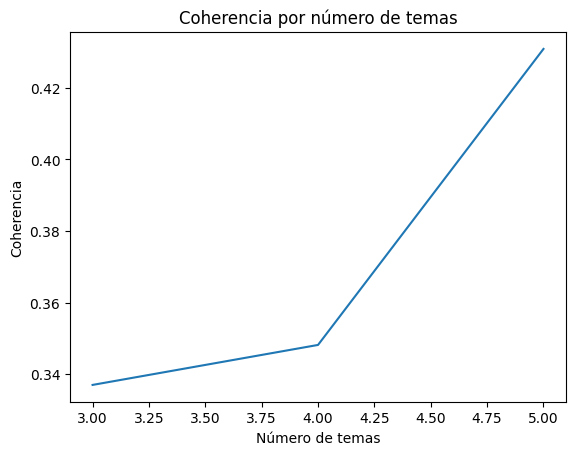
\includegraphics[width=0.6\textwidth]{imagec.png}
        \caption{Coherencia por número de temas}
        \label{fig:coherencia_temas}
    \end{figure}
\end{frame}

\subsection{Distribución de los Temas Identificados}
\begin{frame}{Distribución de los Temas Identificados}
    \begin{figure}[H]
        \centering
        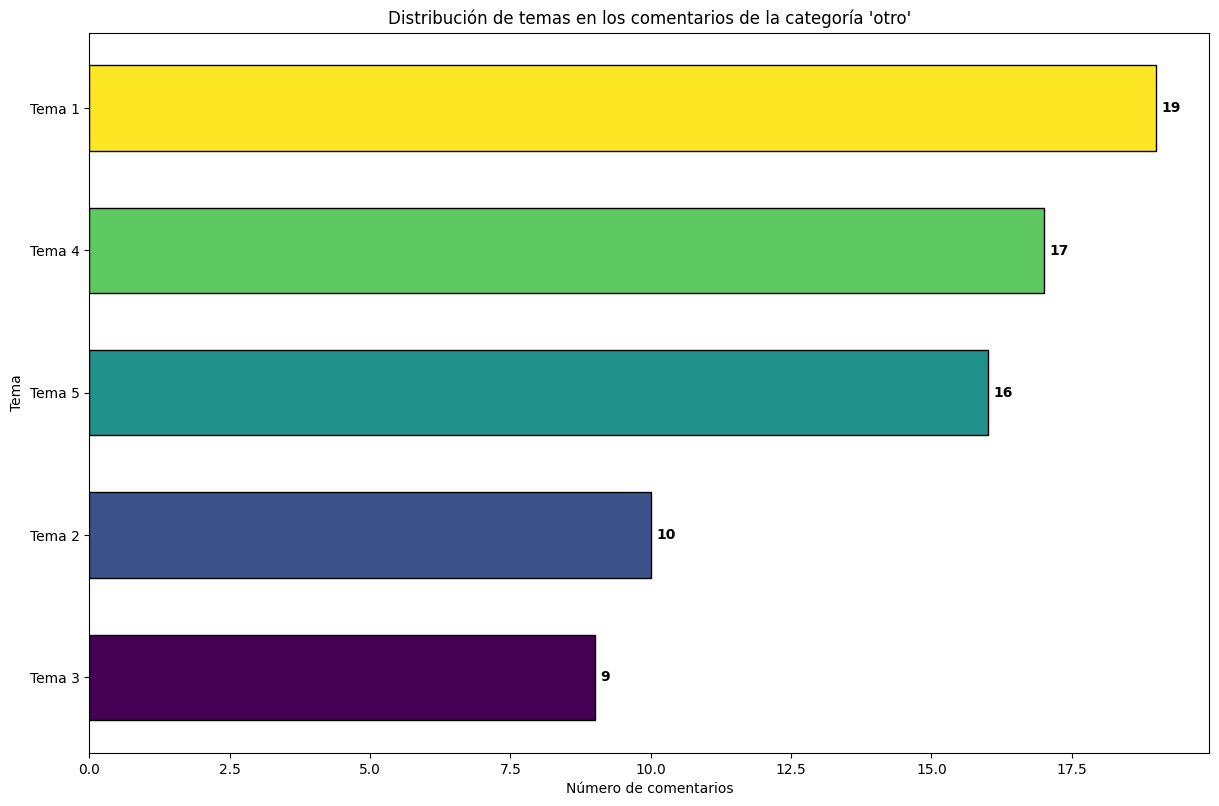
\includegraphics[width=0.8\textwidth]{imaged.png}
        \caption{Distribución de los temas en los comentarios}
        \label{fig:distribucion_temas}
    \end{figure}
\end{frame}

\subsection{Interpretación de los Tópicos}
\begin{frame}{Interpretación de los Tópicos}
    \begin{itemize}
        \item \textbf{Tema 1}: Insatisfacción con el servicio al cliente.
        \begin{itemize}
            \item Palabras clave: decepción, inaceptable, respuesta.
        \end{itemize}
        \item \textbf{Tema 2}: Actitud y comportamiento del personal.
        \begin{itemize}
            \item Palabras clave: grosería, relación, insatisfactorio.
        \end{itemize}
    \end{itemize}
\end{frame}

\begin{frame}{Interpretación de los Tópicos (cont.)}
    \begin{itemize}
        \item \textbf{Tema 3}: Tiempo de espera y rapidez en la atención.
        \begin{itemize}
            \item Palabras clave: espera, minutos, rápido.
        \end{itemize}
        \item \textbf{Tema 4}: Problemas en sucursales y personal.
        \begin{itemize}
            \item Palabras clave: personal, sucursal, inquietud.
        \end{itemize}
        \item \textbf{Tema 5}: Problemas técnicos con aplicaciones y transacciones móviles.
        \begin{itemize}
            \item Palabras clave: aplicación, transacción, fallo.
        \end{itemize}
    \end{itemize}
\end{frame}

\subsection{Recomendaciones}
\begin{frame}{Recomendaciones}
    \begin{itemize}
        \item \textbf{Expansión del análisis} a otros canales de retroalimentación (chats, llamadas, correos electrónicos).
        \item \textbf{Integración de encuestas} de satisfacción instantáneas tras interacciones clave.
        \item \textbf{Desarrollo de modelos predictivos} basados en NPS para anticipar comportamiento de clientes.
    \end{itemize}
\end{frame}

\begin{frame}{Recomendaciones (cont.)}
    \begin{itemize}
        \item \textbf{Exploración de técnicas más avanzadas} de análisis de texto (e.g., BERT, Word2Vec) para mejorar la comprensión semántica.
        \item \textbf{Automatización de la retroalimentación} mediante sistemas que analicen comentarios de forma continua.
        \item \textbf{Futuros estudios académicos y colaboraciones} para mejorar la robustez de los modelos desarrollados.
    \end{itemize}
\end{frame}

% Sección: Anexos
\section*{Anexos}
\begin{frame}{Anexos}
    Los anexos de este trabajo incluyen el código desarrollado en \textbf{Google Colab}, así como las bases de datos. Puedes acceder al código en el siguiente enlace:

    \vfill
    \url{https://colab.research.google.com/drive/1AVMlirkqufPE-BpA9_ZLStWFVA-XSetJ?usp=sharing}
\end{frame}

% Sección: Referencias
\section*{Referencias}
\begin{frame}[allowframebreaks]
    \frametitle{Referencias}
    \footnotesize
    \printbibliography
\end{frame}

\end{document}

